\chapter{Methods}
\begin{itemize}
\item Need to preserve spatial information for symbolic front-end
\item Need disentangled latent space for symbolic front-end
\item This may be summarised as needing to be able to deduce the object type and its location solely from the latent space representation
\item Explain degree of freedom here (disentangled filters, or disentangled neurons, or something else?)
\item This is unexplored territory - we decide what the reasonable architecture should be, then evaluate it in the results section
\item As far as we know, this section contains the first considerations of a convolutional variational latent space
\end{itemize}

\label{ch:methods}


%
%
%
%
%
\section{Single Latent Filter}

\begin{itemize}
\item As mentioned, the type and position of an object must be preserved in the latent space
\item This may be achieved by using a single latent filter, with the object type corresponding to the value of the weighted sum of the neuron.
\item (Recall that no activation function is used for these layers)
\end{itemize}

\subsection{Architecture}
\begin{itemize}
\item The convolutional mean $\mu$ and variance $\sigma^2$, both of shape $(k, m, n)$, are sampled using ... cite reparameterisation trick here... to give the latent space of shape $(k, m, n)$. 
\item The proposed architecture is shown in Figure (\ref{fig:latent_image_architecture})
\end{itemize}

\begin{figure}[H]
\centering
\captionsetup{justification=centering}
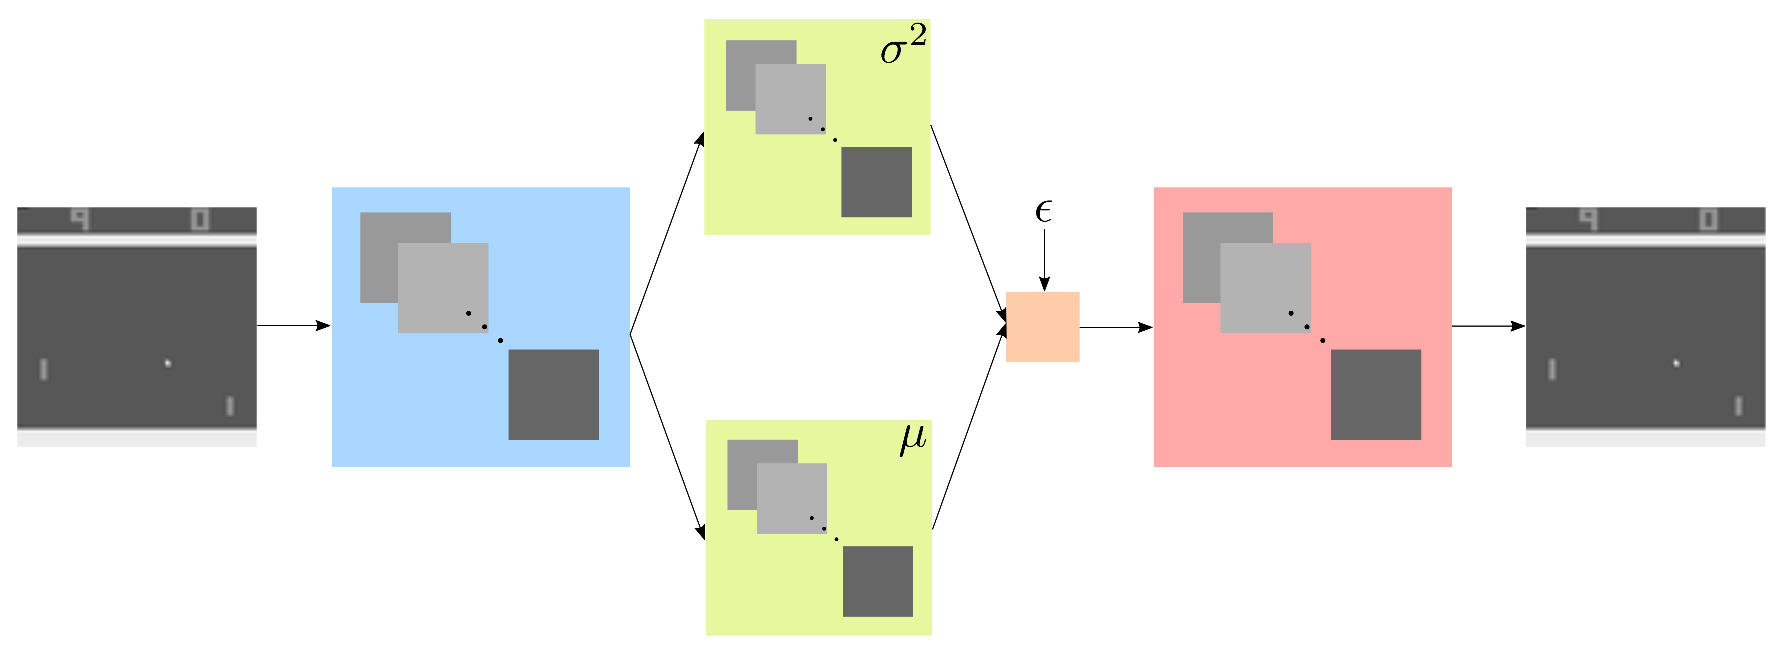
\includegraphics[scale=0.58]{methods/latent_image_architecture.eps}
\caption{The single latent filter architecture. \textbf{Blue:} An arbitrary amount of convolutional layers. \textbf{Green:} The latent mean $\vec{\mu}$ and variance $\vec{\sigma}^2$, which are both volumes of shape $(k, m, n)$. \textbf{Orange:} A single latent filter of shape $(1, m, n)$ sampled component-wise from $\vec{\mu}$ and $\vec{\sigma}^2$. \textbf{Red:} The corresponding deconvolutional layers.}
\label{fig:latent_image_architecture}
\end{figure}

\begin{figure}[h!]
\centering
\captionsetup{justification=centering}
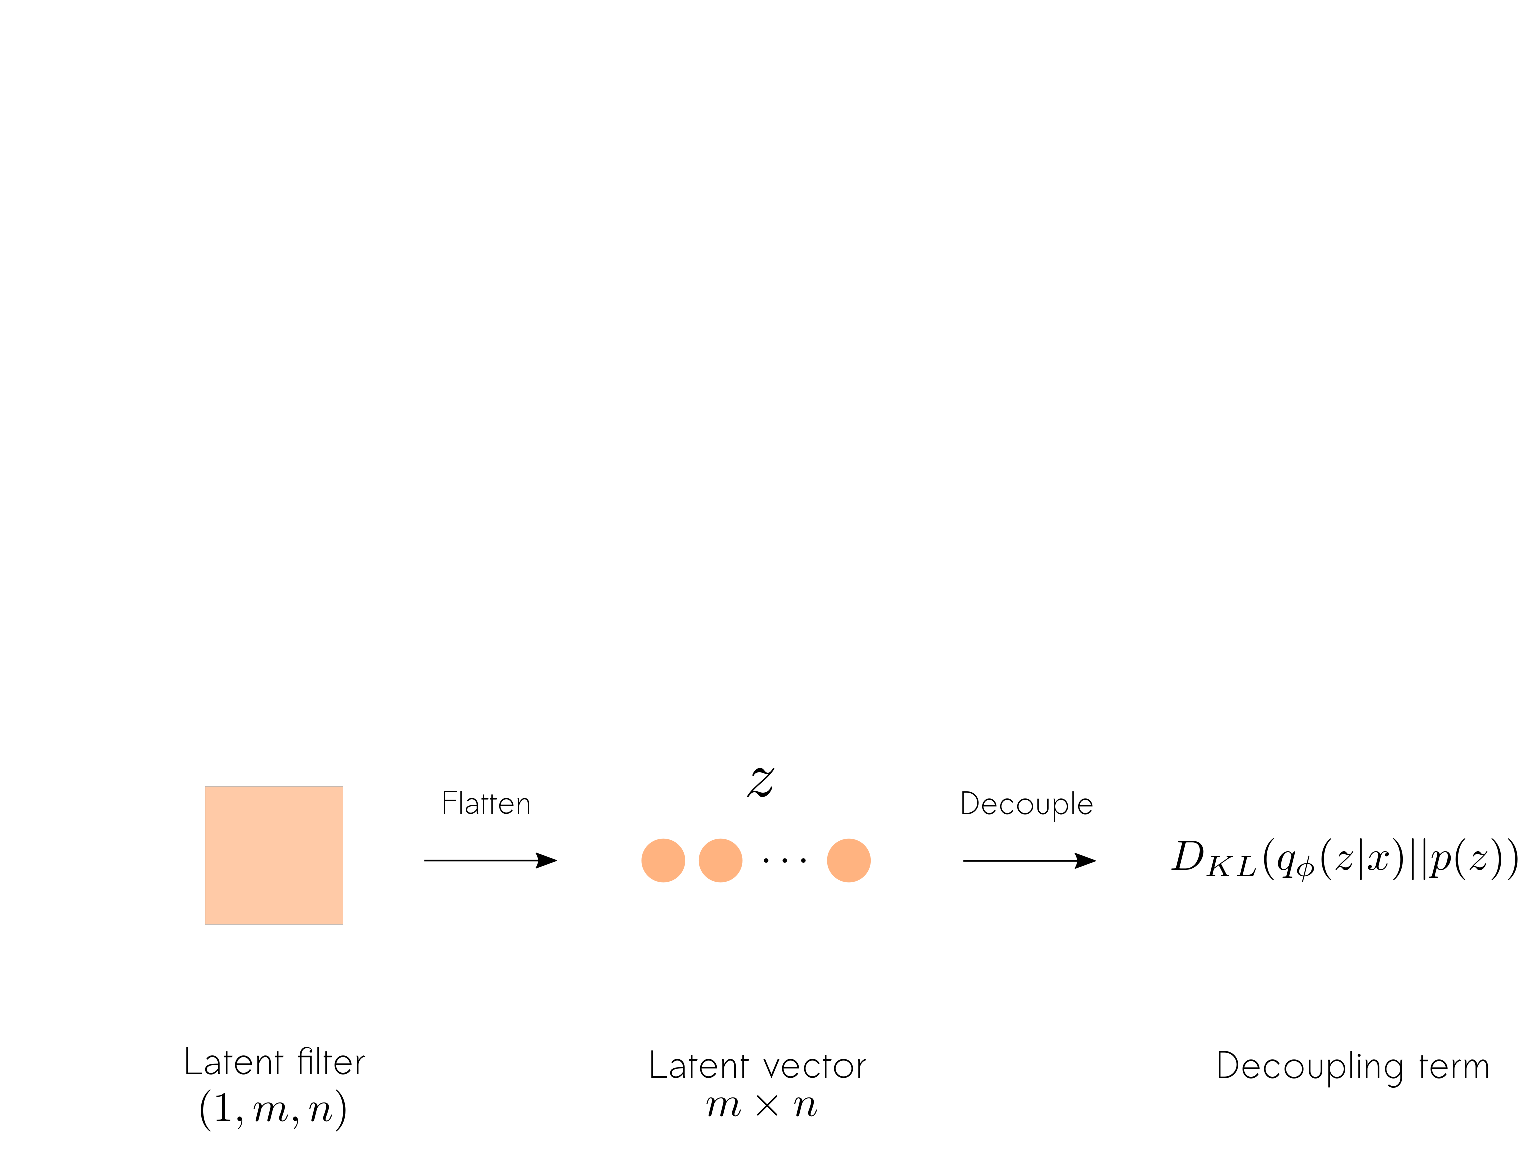
\includegraphics[scale=0.6]{methods/latent_image_flattening_latent_space.eps}
\caption{Caption.}
\label{fig:latent_image_flattening_latent_space}
\end{figure}

\subsection{Derivation}
\begin{itemize}
\item The latent filter of shape $(1, m, n)$ is flattened 
\end{itemize}

%
%
%
%
%
\section{Disentangling Latent Neurons}
\lipsum[2]
\subsection{Architecture}
\begin{figure}[h!]
\centering
\captionsetup{justification=centering}
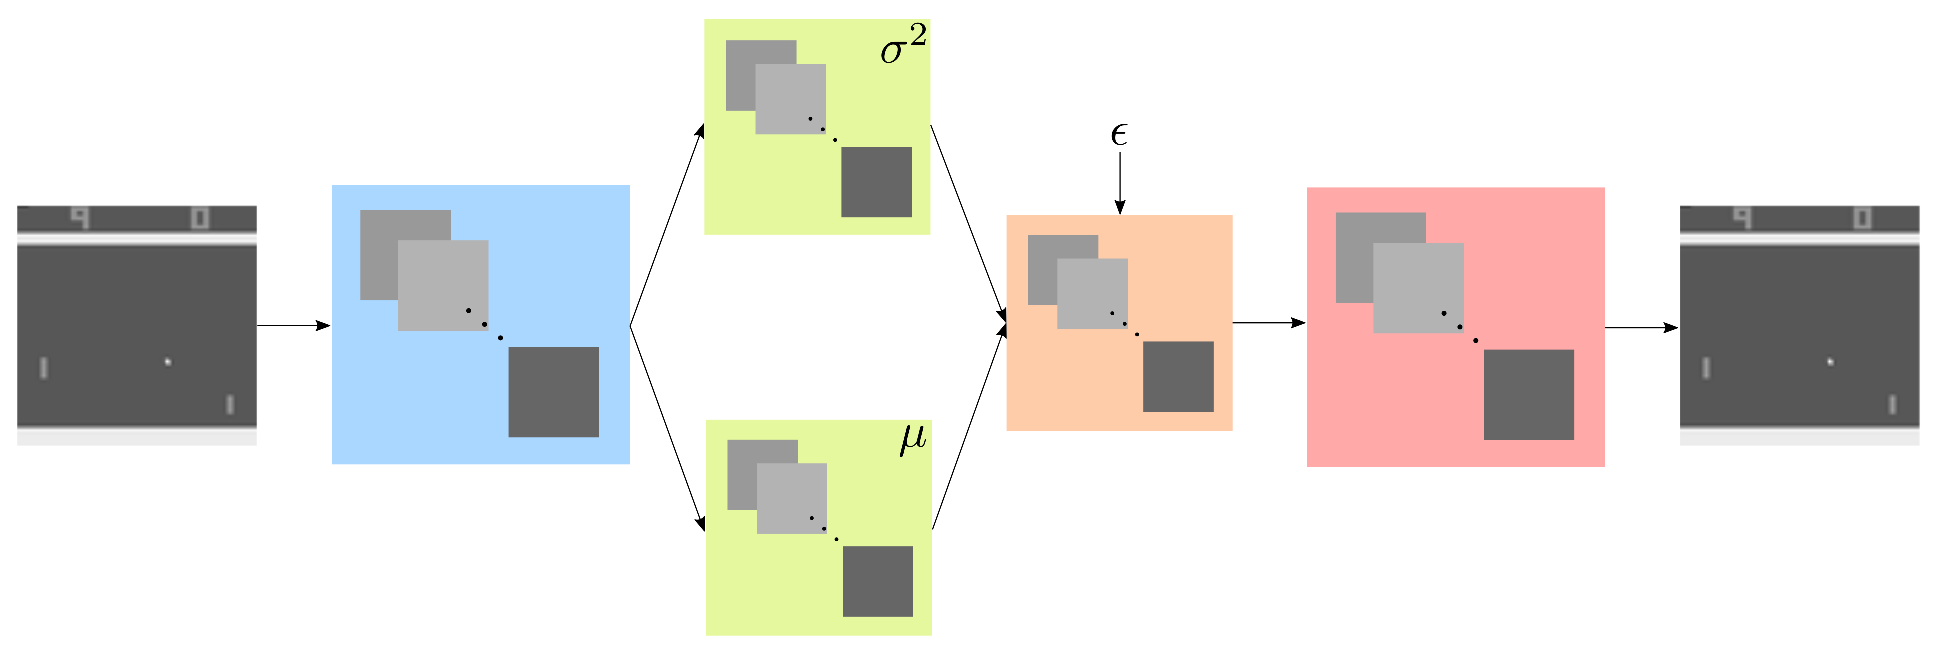
\includegraphics[scale=0.55]{methods/decoupling_indiscriminately_horizontal.eps}
\caption{Caption.}
\label{fig:decoupling_indiscriminately_horizontal}
\end{figure}

\begin{figure}[h!]
\centering
\captionsetup{justification=centering}
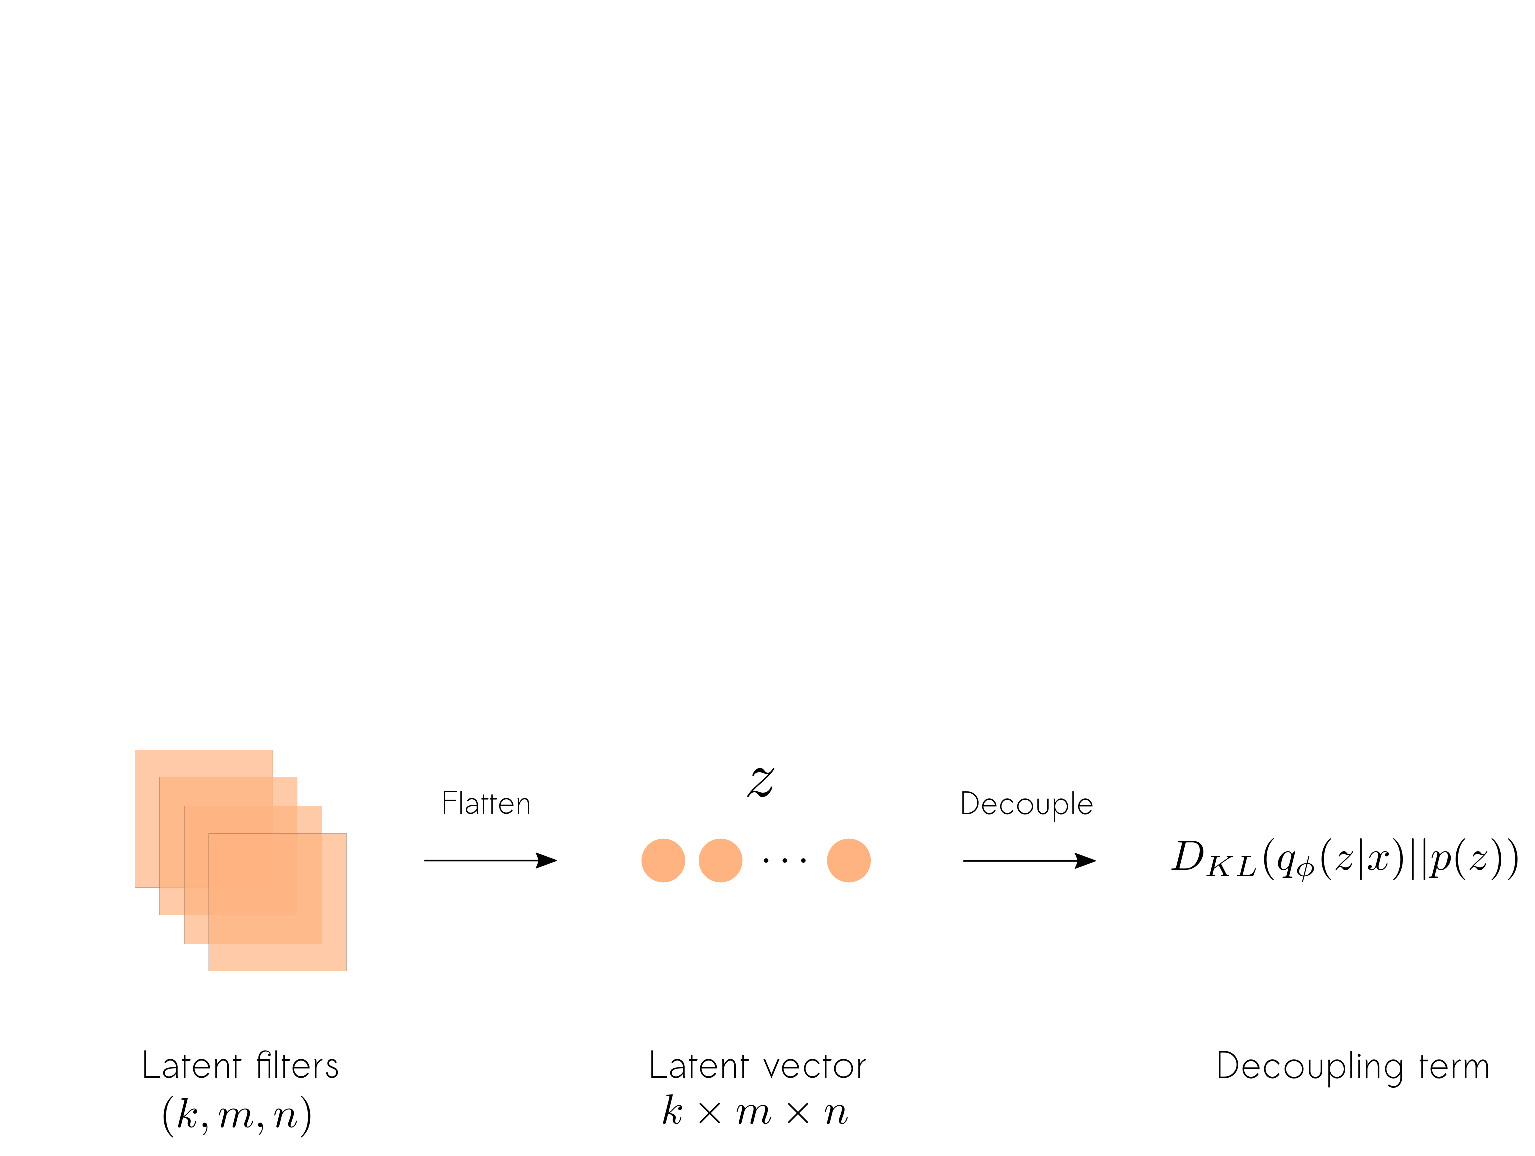
\includegraphics[scale=0.6]{methods/decoupling_indiscriminately_flattening_latent_space.eps}
\caption{Caption.}
\label{fig:decoupling_indiscriminately_flattening_latent_space}
\end{figure}

\subsection{Derivation}



%
%
%
%
%
\section{Disentangling Latent Filters Using Averages}
\lipsum[2]
\subsection{Architecture}
\begin{figure}[H]
\centering
\captionsetup{justification=centering}
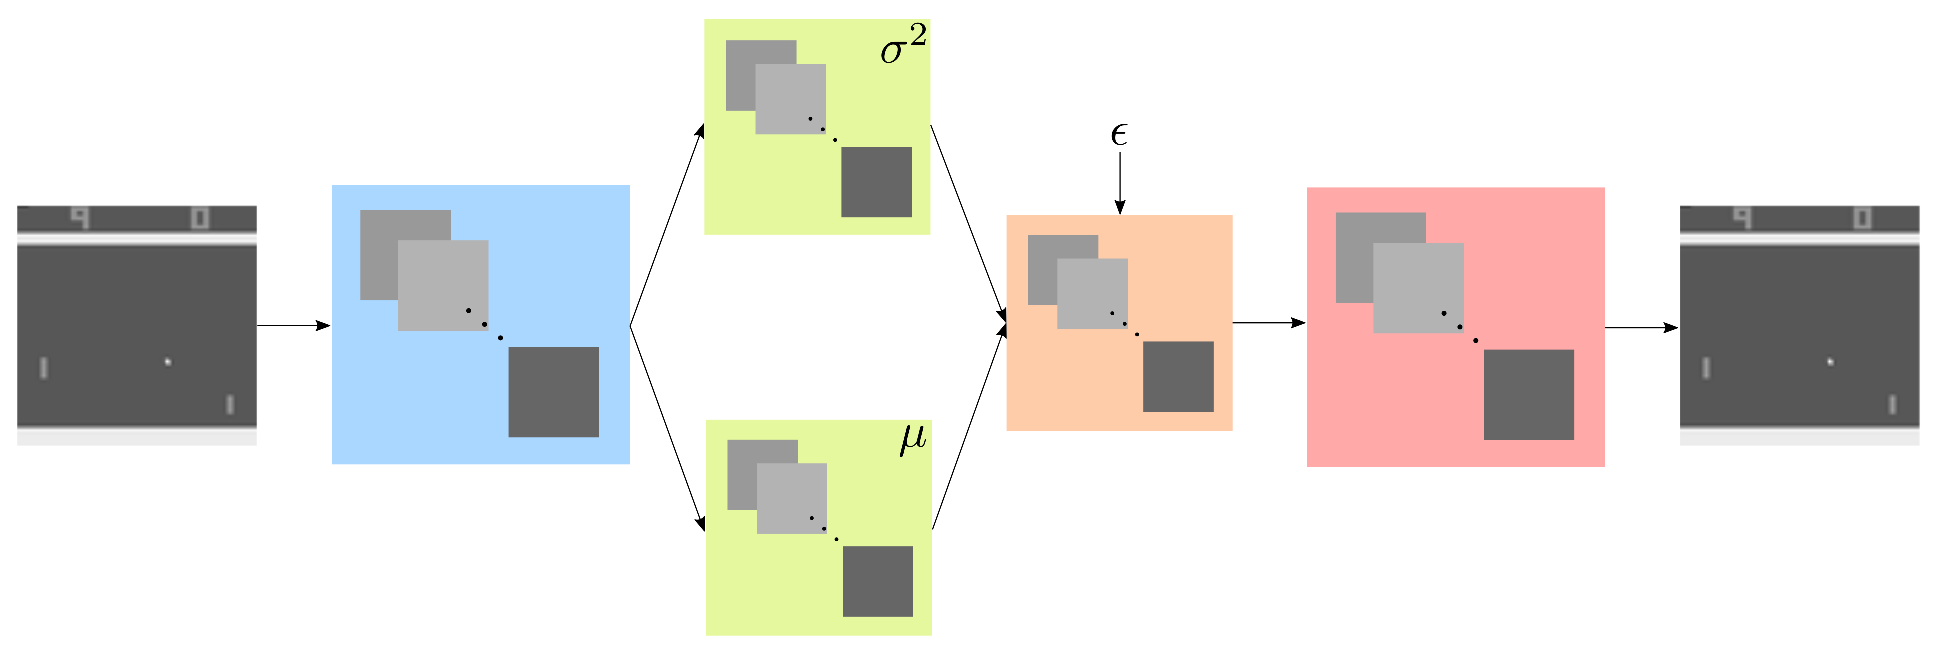
\includegraphics[scale=0.55]{methods/decoupling_indiscriminately_horizontal.eps}
\caption{Caption.}
\label{fig:decoupling_indiscriminately_horizontal}
\end{figure}

\begin{figure}[H]
\centering
\captionsetup{justification=centering}
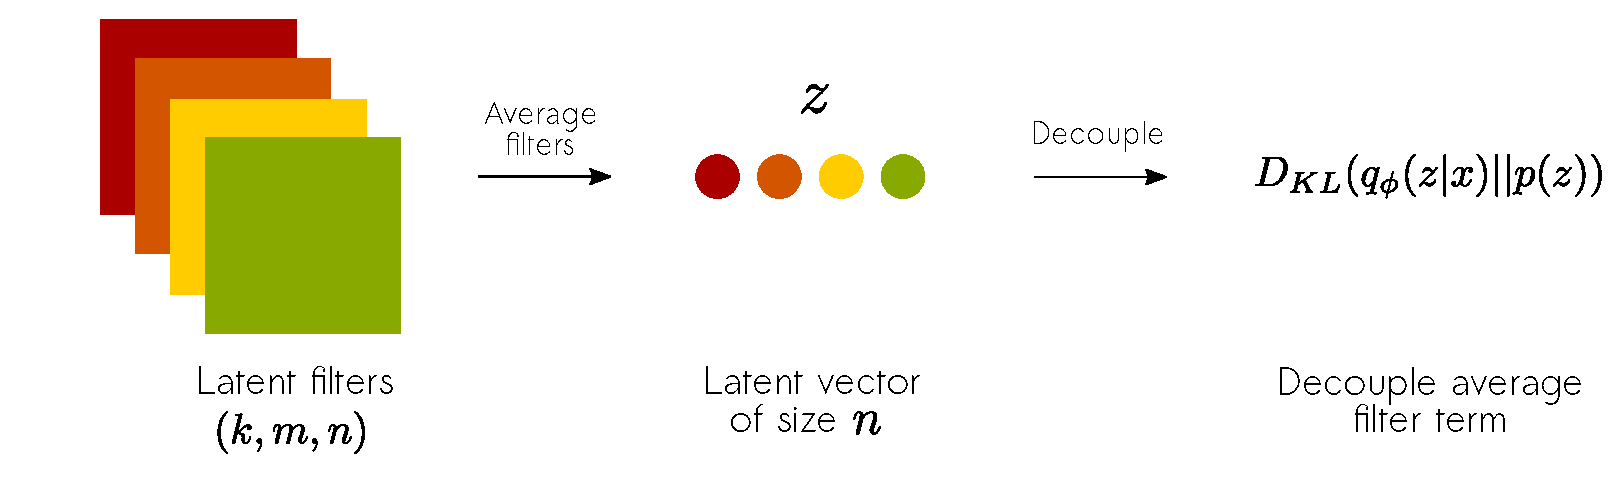
\includegraphics[scale=0.6]{methods/decoupling_averages_latent_space.eps}
\caption{Caption.}
\label{fig:decoupling_averages_latent_space}
\end{figure}

\subsection{Derivation}

%
%
%
%
%
\section{Decoupling Latent Filters Using Weighted-Averages}
\lipsum[2]
\subsection{Architecture}
\subsection{Derivation}

%
%
%
%
%
\section{Separating Colour Spaces}
\lipsum[2]
\subsection{Architecture}
\subsection{Derivation}

%
%
%
%
%
\section{Orthogonal Convolutions}
\lipsum[2]
\subsection{Architecture}
\begin{figure}[h!]
\centering
\captionsetup{justification=centering}
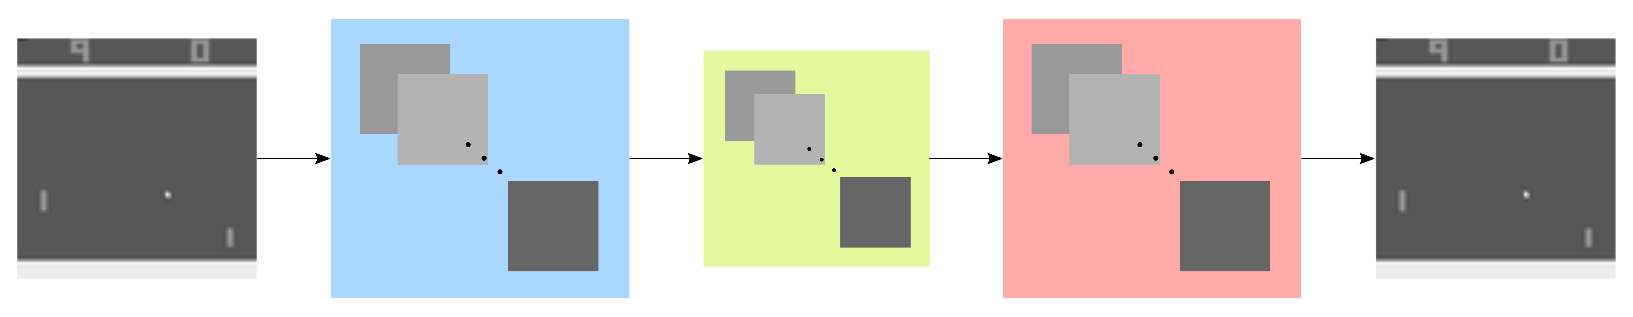
\includegraphics[scale=0.63]{methods/orthogonal_convolutions_archiecture.eps}
\caption{Caption.}
\label{fig:orthogonal_convolutions_archiecture}
\end{figure}

\subsection{Derivation}

%
%
%
%
%
\section{Winner Takes All}
\lipsum[2]
\subsection{Architecture}
\subsection{Derivation}
